\documentclass[]{article}

% Options for packages loaded elsewhere
\PassOptionsToPackage{unicode}{hyperref}
\PassOptionsToPackage{hyphens}{url}
\PassOptionsToPackage{dvipsnames,svgnames,x11names}{xcolor}

\usepackage{xcolor}
\usepackage[margin=1in]{geometry}
\usepackage{amsmath,amssymb}
\setcounter{secnumdepth}{-\maxdimen} % remove section numbering
\usepackage{iftex}
\ifPDFTeX
  \usepackage[T1]{fontenc}
  \usepackage[utf8]{inputenc}
  \usepackage{textcomp} % provide euro and other symbols
\else % if luatex or xetex
  \usepackage{unicode-math} % this also loads fontspec
  \defaultfontfeatures{Scale=MatchLowercase}
  \defaultfontfeatures[\rmfamily]{Ligatures=TeX,Scale=1}
\fi
\usepackage{lmodern}

% Use upquote if available, for straight quotes in verbatim environments
\IfFileExists{upquote.sty}{\usepackage{upquote}}{}
\IfFileExists{microtype.sty}{% use microtype if available
  \usepackage[]{microtype}
  \UseMicrotypeSet[protrusion]{basicmath} % disable protrusion for tt fonts
}{}

\makeatletter
\@ifundefined{KOMAClassName}{% if non-KOMA class
  \IfFileExists{parskip.sty}{%
    \usepackage{parskip}
  }{% else
    \setlength{\parindent}{0pt}
    \setlength{\parskip}{6pt plus 2pt minus 1pt}}
}{% if KOMA class
  \KOMAoptions{parskip=half}}
\makeatother

\usepackage{graphicx}
\makeatletter
\newsavebox\pandoc@box
\newcommand*\pandocbounded[1]{% scales image to fit in text height/width
  \sbox\pandoc@box{#1}%
  \Gscale@div\@tempa{\textheight}{\dimexpr\ht\pandoc@box+\dp\pandoc@box\relax}%
  \Gscale@div\@tempb{\linewidth}{\wd\pandoc@box}%
  \ifdim\@tempb\p@<\@tempa\p@\let\@tempa\@tempb\fi% select the smaller of both
  \ifdim\@tempa\p@<\p@\scalebox{\@tempa}{\usebox\pandoc@box}%
  \else\usebox{\pandoc@box}%
  \fi%
}
% Set default figure placement to htbp
\def\fps@figure{htbp}
\makeatother
\setlength{\emergencystretch}{3em} % prevent overfull lines
\providecommand{\tightlist}{%
  \setlength{\itemsep}{0pt}\setlength{\parskip}{0pt}}
\usepackage{bookmark}
\IfFileExists{xurl.sty}{\usepackage{xurl}}{} % add URL line breaks if available
\urlstyle{same}

\hypersetup{
  pdftitle={ISTG1003 prosjekt: Tittel (gi projektet en informativ tittel)},
  pdfauthor={Emma Nordli, Magnus Kåsa Morisbakk, Patrick Alund},
  colorlinks=true,
  linkcolor={black},
  filecolor={black},
  citecolor={black},
  urlcolor={blue},
  pdfcreator={LaTeX via pandoc}
}

% --- NY KOMMANDO FOR FORSIDEN ---
\newcommand{\HRule}{\rule{\linewidth}{0.5mm}} 

% ==========================================
% NYTT: BIBLATEX CONFIGURATION FOR ISTG1003
% ==========================================
\usepackage[norsk]{babel} % Sikrer at dokumentet forstår norsk språk
\usepackage{csquotes}     % Hjelper biblatex med korrekte sitattegn på norsk
\usepackage[backend=biber, style=apa, langid=norsk]{biblatex}
\addbibresource{references.bib} % Sørg for at filen din heter nøyaktig references.bib
% ==========================================

\begin{document}

% Henter inn den nye forsiden din
% Inspired by title template from ShareLaTeX Learn; Gubert Farnsworth & John Doe
% Edited by Jon Arnt Kårstad, NTNU IMT

\begin{titlepage}
\vbox{ }
\vbox{ }
\begin{center}
% Upper part of the page

\includegraphics[width=0.40\textwidth]{Images/NTNU_logo.png}\\[1cm]
\textsc{\LARGE Institutt for informasjonssikkerhet og kommunikasjonsteknologi}\\[1.5cm]
\textsc{\Large ISTG1003 - Statistikk}\\[0.5cm]
\vbox{ }

% Title
\HRule \\[0.4cm]
{ \huge \bfseries Prosjekt: Tittel}\\[0.4cm]
\HRule \\[1.5cm]

% Author
\large
\textbf{Gruppe 1:}\\
Emma Nordli \\
Magnus Kåsa Morisbakk \\
Patrick Alund \\

\vfill

% Bottom of the page

\end{center}
\end{titlepage}
\newpage

% --- INNHOLDSFORTEGNELSE ---
\tableofcontents
\newpage

Rapporten gir maks 50 poeng. Fordeling av poengene vises for hver del.
Hver del blir vurdert etter

\begin{itemize}
\tightlist
\item
  faglig nivå
\item
  korrekthet
\item
  presentasjon og lesbarhet
\end{itemize}

% Her henter vi inn alle underfilene
\section{Sammendrag/Abstract (max 500 ord) (10 poeng)}\label{sammendragabstract-max-500-ord-10-poeng}

Formålet med sammendraget er å gi en kort og presis oppsummering av
prosjektet deres. Det er en selvstendig tekst som plasseres før selve
rapporten begynner (men skriv den til slutt). Sammendraget bør inneholde
følgende deler:

\begin{enumerate}
\def\labelenumi{\arabic{enumi}.}
\tightlist
\item
  Start med å tydelig beskrive formålet med prosjektet. Hvilket problem
  forsøker dere å løse? Hvilket spørsmål ønsker dere å besvare? Beskriv
  forskningsspørsmålet/hypotesen. Det er viktig å være kortfattet og
  konkret.
\item
  Beskriv dataene dere brukte. Inkluder lenken til datasettet her.
  Hvilket datasett benyttet dere? Deklarer størrelse på datasettet
  (antall observasjoner, antall variabler), typer variabler og
  responsvariabel.
\item
  Beskriv metodene: Hvordan analyserte dere dataene? Hvilke verktøy,
  teknikker eller metoder brukte dere? Regresjon, klassifisering,
  klyngeanalyse? Vær spesifisk, men unngå for mange detaljer.
\item
  Oppsummer de viktigste funnene. I hoveddelen av sammendraget skal dere
  oppsummere de viktigste resultatene fra prosjektet og kort tolke dem
  (altså, hva betyr resultatene?). Fremhev de mest betydningsfulle
  funnene, og gi nok informasjon til at leseren får et inntrykk av hva
  dere har oppdaget.
\item
  (Valgfritt) Fremhev betydningen av resultatene. Forklar hvorfor
  og/eller hvordan funnene dine er viktige. Fremhev eventuelle nye eller
  uventede funn, og forklar hvordan de bidrar til økt forståelse av
  temaet.
\end{enumerate}
\section{Introduksjon (10 poeng)}\label{introduksjon-10-poeng}
Vårt prosjekt tar for seg datasettet \textit{Titanic-Dataset.csv} hentet fra kaggle. Datasesettet dokumenterer informasjon knyttet til 891 passasjerer ombord Titanic i 1912 \parencite[]{titanic_dataset}.

Problemstillingen vi har tatt for oss er todelt. Datasettet mangler data knyttet til enkelte av radene, vi ønsker derfor å se om vi kan benytte multippel regresjon for å anslå passasjerers alder basert på forhåndbestemte faktorer som klasse, kjønn og størrelse på familie. 

Det andre vi ønsker å ta for oss er å estimere sannsynligheten for at en passasjer har overlevd hendelsen eller ikke ved bruk av klassifisering. Hvilke faktorer kan ha utgjort forskjellen på liv og død? Vi ønsker å finne en metode som gir et nøyaktig og realistisk bilde av sjansen for passasjerers overlevelse.
\section{Beskrivende dataanalyse (5 poeng)}\label{beskrivende-dataanalyse-5-poeng}
Datasettet består av totalt 2906 observasjoner. For analysen, så har vi valgt å fokusere de følgende variablene; pris (realSum), avstand til sentrum (dist), kapasitet (person\textunderscore capacity) og tilfredsstillhet (guest\textunderscore satisfaction\textunderscore overall), da det er disse variablene som er mest relevant for våre problemstillinger.

En gjennomgang av datasettet, viser at gjenomsnittsprisen for en natt for to personer, en helg i Lisboa er 240 euro, medianprisen er noe lavere på 227. Et høyere gjennomsnitt indikerer en noe høyreskev fordeling. Det er en håndful dyrere utleieboliger som drar opp prisen. Leilighetene ligger i snitt ganske nært sentrum, med en avstand på 1.97km, og gjestene er generelt svært fornøyde med en median på 93/100 for gjestetilfredstillhet. 


\paragraph{Prisfordeling} \mbox{} \\
Ettersom at pris er hovedfokuset i regresjonsanalysen, har vi undersøkt fordelingen ved bruk av histogram. Fordelingen av av \textbf{realSum} bekrefter observasjonen om høyreskjevhet. Den største andelen av leilighetene koster under 300  euro, mens den lange "halen" som strekker seg mot høyre er de få dyrere og mer ekslusive leilighetene.

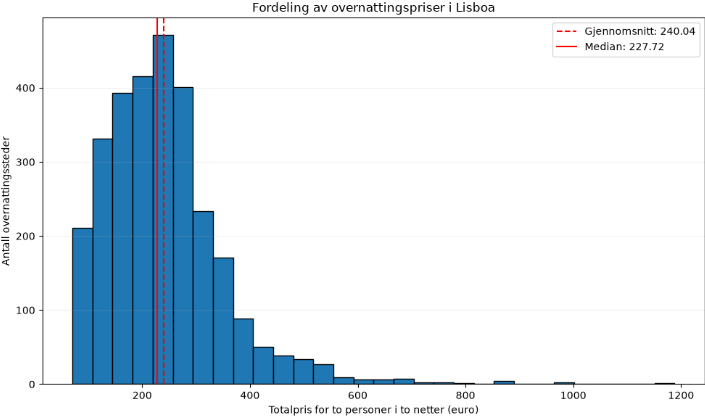
\includegraphics[]{Images/fordeling_overnattingspriser.png}

Her bør du gjennomføre en kort deskriptiv dataanalyse for å få en
oversikt over datasettet. Det betyr at man lager noen visualiseringer
for å forstå dataene bedre, og at man beregner noen enkle ting. Fokuser
på det som er relevant for modelleringen, og bruk sunn fornuft. For mye
detaljer eller figurer uten forklaring og tydelige akseetiketter er ikke
nyttige for leseren.

\paragraph{Sammenhenger} \mbox{}\\
Vi har benyttet spredningsdiagram som å undersøke sammenhengen mellom pris og beliggenhet. Diagrammet viser at leilighetene som ligger nærmest sentrum har både den høyeste gjennomsnittsprisen og størst variasjon og pris.

Variabelen \textbf{person\textunderscore capacity} har som forventet høyest korrelasjon med pris på (r = 0.567). Avstand til sentrum (\textbf{dist}) har overraskende nok en negativ korrelasjon på (r = -0.146), og gjestefilfredstillhet har en positiv korrelasjon på (r = 0.148).


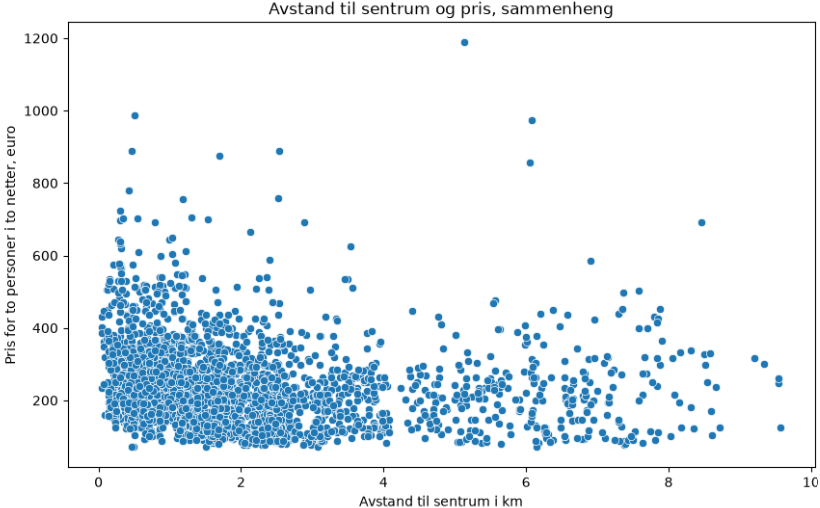
\includegraphics[]{Images/avstand_til_sentrum_pris_sammenheng.png}

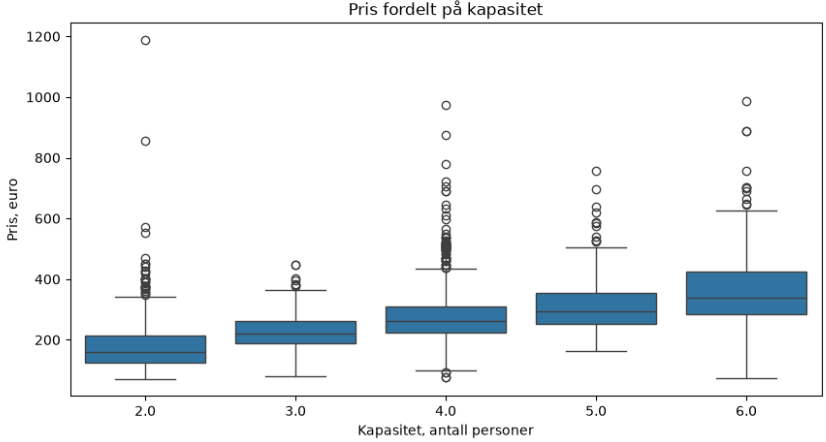
\includegraphics[]{Images/boksplott_pris_gruppert_kapasitet.png}

Du kan for eksempel:

\begin{itemize}
\tightlist
\item
  Presentere deskriptiv statistikk, som gjennomsnitt, median,
  standardavvik og varians, for å beskrive datasettets sentraltendens,
  variasjon og fordeling.
\item
  Bruke spredningsdiagrammer (scatter plots) og korrelasjonsmatriser for
  å undersøke sammenhenger mellom ulike variabler.
\item
  Bruke histogrammer for å vise fordelingen til relevante variabler.
\item
  Bruke boksplott (box plots) for å undersøke fordeling, variasjon og
  eventuelle uteliggere.
\end{itemize}

Resultatene bør forklares i teksten, med særlig fokus på funn som kan
være relevante for den videre modelleringen. Skriv en kort legende under
hver grafikk, slik at det blir tydelig hva grafikken viser.
\section{Metoder (10 poeng)}\label{metoder-10-poeng}

\subsection{1. Multippel lineær regresjon} 
For å løse den første delen av problemstilling, estimering av manglende aldersdata hos enkelte rader, benytter vi multippel lineær regresjon og estimering med OLS. Ettersom at alder er en kontinuerlig variabel, så er lineær regresjon en egnet metode for å undersøke sammenhengen mellom alder og forklaringsvariablene.

% $$Y_i = \beta_0 + \beta_1 x_{1i} + \beta_2 x_{2i} + \dots + \beta_p x_{pi} + e_i$$

\paragraph{Validering} \mbox{} \\
Determinasjonskoeffisient (justert $R^2$) benyttes for å si hvor stor andel av variansen i alder som kan forklares av de valgte prediktorene. \\
HKoeffisienten til hver prediktor evalueres mot et signifikansnivå på 0.05 for å avgjøre om sammenhengen mellom prediktoren og alder er statistisk signifikant. \\
To grafiske analyser utføres for å validere at forutsetningene til OLS er oppfylt:
\begin{itemize}
    \item Scatterplot: Undersøke om sammenhengen er lineær.
    \item Q-Q-plott: Undersøke om residualene er normalfordelte.
\end{itemize}

\subsection{2. Klassifisering}

\paragraph{Begrensninger ved metodene}
\begin{itemize}
    \item Fjerning av rader som har manglende data, kan potensielt forårsake skjevheter i datasettet som modellene evalueres etter.
    \item Ettersom at OLS er uavgrenset, så kan det forekomme negative aldersverdier dersom en passasjer har en kombinasjon av flere prediktorer (eks. høyt antall pårørende).
\end{itemize}

\section{Resultater (10 poeng)}\label{resultater-10-poeng}

\begin{enumerate}
\def\labelenumi{\arabic{enumi}.}
\item
  Presenter resultatene på en tydelig og strukturert måte. Dette kan for
  eksempel gjøres ved hjelp av tabeller, grafer eller andre
  visualiseringer som gjør funnene lettere å forstå.
\item
  Tolk resultatene. Tolkningen bør tilpasses regresjons-,
  klassifiserings- eller klyngeanalyse-oppgaven du har valgt.
\item
  Diskuter begrensninger og forbehold som er viktige å ta hensyn til når
  resultatene skal tolkes. Dette kan for eksempel være begrensninger ved
  datasettet, modellene eller evalueringsmetodene.
\item
  (Valgfritt) Se på mulige videre analyser. Beskriv eventuelt
  alternative eller forbedrede metoder som kunne vært brukt for å
  analysere dataene i fremtiden, og hvordan disse potensielt kunne gitt
  ytterligere innsikt.
\end{enumerate}
\section{Diskusjon og konklusjon (5 poeng)}\label{diskusjon-og-konklusjon-5-poeng}

Oppsummer de viktigste funnene fra prosjektet deres. Hva fant du ut, og
hvilke var de viktigste innsiktene du fikk gjennom analysen? Fokuser på
de mest relevante resultatene fra modelleringen og analysen.

\newpage
\section{Deklarasjon om KI-hjelpemidler (maks 1 side -- teller ikke til de 10 sidene i rapporten)}\label{deklarasjon-om-ki-hjelpemidler}

Besvar følgende sprørsmål:

1.) Har det i utarbeidingen av denne rapporten blitt anvendt KI-baserte
hjelpemidler? Hvis ja, beskriv hvilke verktøy dere brukte (Copilot, NTNU
GPT,\ldots).

2.) Er en eller flere av ideene eller fremgangsmåtene i oppgaven
foreslått av KI? Hvis ja, beskriv her:

3.) Tekst: Har du brukt KI for

\begin{enumerate}
\def\labelenumi{\alph{enumi})}
\tightlist
\item
  Stavekontroll?
\item
  Språkvask?
\item
  Tekstgenerering?
\item
  Skriveassistanse.
\end{enumerate}

Hvis du svarer ja på minst en av a)-d), spesifiser bruken her:

4.) Kode og algoritmer: Programmeringsassistanse. Er deler av
koden/algoritmene som i) fremtrer direkte i rapporten eller ii) har
blitt anvendt for produksjon av resultater slik som figurer, tabeller
eller tallverdier blitt generert av KI? Hvis ja, spesifiser bruken her:

5.) Bilder og figurer, bildegenerering. Er ett eller flere av
bildene/figurene i rapporten blitt generert av KI? Hvis ja, beskriv
bruken her:

6.) Beskrive alle andre aspekter av arbeidet som KI ble brukt til.
Beskriv her:

7.) Ved innlevering av prosjektet deklarerer vi at vi er kjent med NTNUs
regelverk: Det er ikke tillatt å generere besvarelser eller tekst ved
hjelp av KI og levere den helt eller delvis som eget arbeid. Vi har
derfor redegjort for all anvendelse av KI enten direkte i rapporten,
eller her. Svar her:

\newpage
% --- OPPDATERT: SEKSJON FOR REFERANSER ---
% Siden du har en underfil som heter "8. Referanser og kode.tex", henter vi den inn først.
\section{Referanser og kode (teller ikke til de 10 sidene i rapporten)}\label{referanser-og-kode}

Her kan dere legge til alle referanser og kode som dere har brukt for å
generere resultatene i rapporten.

% Dette genererer selve litteraturlisten automatisk rett under innholdet i filen over:
\printbibliography[heading=none] 

\end{document}
